% fig_dt_flag_rates.tex
% TR-45: DT flag rates by k_ibr region
%
% Grouped bar chart:
%   Regions: k<0.06 (33), 0.06≤k<0.10 (91), k≥0.10 (833)
%   FP rates: 18.18%,  0.00%,  0.00%
%   FN rates:  0.00%, 15.38%,  1.92%

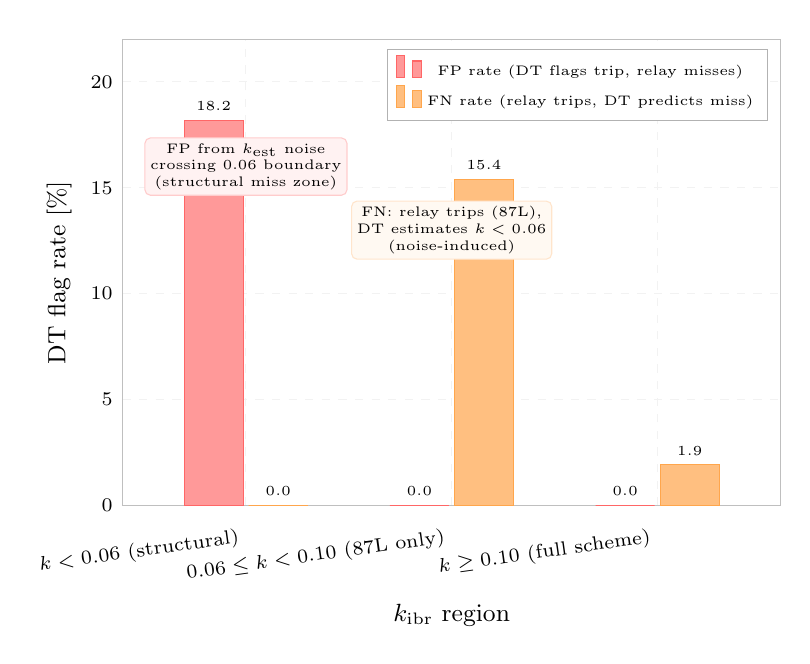
\begin{tikzpicture}
\begin{axis}[
  name         = flagax,
  width        = 0.82\textwidth,
  height       = 7.5cm,
  ybar,
  bar width    = 0.75cm,
  xlabel       = {$k_\mathrm{ibr}$ region},
  ylabel       = {DT flag rate [\%]},
  xlabel style = {font=\small},
  ylabel style = {font=\small},
  ymin=0, ymax=22,
  ytick        = {0,5,10,15,20},
  yticklabel style={font=\scriptsize},
  xtick        = {1,2,3},
  xticklabels  = {$k<0.06$ (structural),
                  $0.06\leq k<0.10$ (87L only),
                  $k\geq0.10$ (full scheme)},
  xticklabel style={font=\scriptsize, rotate=8, anchor=north east},
  tick style   = {draw=none},
  axis line style={gray!50},
  grid         = major,
  grid style   = {gray!10, dashed},
  nodes near coords,
  nodes near coords style={font=\tiny, anchor=south},
  every node near coord/.append style={
    /pgf/number format/.cd, fixed, fixed zerofill, precision=1
  },
  legend style={at={(0.98,0.98)}, anchor=north east, font=\tiny,
                draw=gray!60, fill=white},
  enlarge x limits=0.30,
  clip=false,
]

%% FP rates
\addplot[fill=red!40, draw=red!60]
  coordinates {(1,18.18) (2,0.00) (3,0.00)};
\addlegendentry{FP rate (DT flags trip, relay misses)}

%% FN rates
\addplot[fill=orange!50, draw=orange!70]
  coordinates {(1,0.00) (2,15.38) (3,1.92)};
\addlegendentry{FN rate (relay trips, DT predicts miss)}

%% Interpretation annotations
\node[draw=red!20, fill=red!5, rounded corners=2pt,
      font=\tiny, inner sep=2pt, align=center]
  at (axis cs:1, 16)
  {FP from $k_\mathrm{est}$ noise\\
   crossing 0.06 boundary\\
   (structural miss zone)};

\node[draw=orange!20, fill=orange!5, rounded corners=2pt,
      font=\tiny, inner sep=2pt, align=center]
  at (axis cs:2, 13)
  {FN: relay trips (87L),\\
   DT estimates $k<0.06$\\
   (noise-induced)};

\end{axis}
\end{tikzpicture}
